\documentclass[12pt, letterpaper]{article}
\usepackage[utf8]{inputenc}
\usepackage{longtable}
\usepackage{graphicx}
\graphicspath{ {images/} }

\title{Recognition of emotions in speech:\\overview and implementation}
\author{Aydar Musin\\Supervisor: prof. Maxim Talanov}
\date{June 2015, Innopolis University}

\begin{document}

\begin{titlepage}
\maketitle
\end{titlepage}

\begin{abstract}
In this paper will be considered research on recognition of emotions in speech, distinguished their techniques, advantages and disadvantages. Then will be offered own simple implementation of the recognition system.
\end{abstract}

\section{Introduction}

Speech emotion recognition has many application areas. More evident of them: robots and improving the quality of customer service.

If robot has ability to emotional speech generating, it will help him to interact with people better. Because understanding of speech emotion recognition gives understanding how to generate emotional speech. And robots with emotional speech are more people-friendly. Also, speech emotion recognition can improve the robot's decision-making system. Because there are situations when a robot needs to take into account human emotions. %Привести пример!!!!!

Closer to reality application of this system is within an estimation of customer service quality. For example, call-centers have records of conversations. And for operator's work estimation we can identify expressive conversations and analyze them.

There are many research where described dependencies between human emotions and acoustic characteristics. Main differences between them in using different:
\begin{itemize}
	\item Acoustics characteristics
	\item Features
	\item Classification techniques
	\item Recognizable emotions
\end{itemize}

The main goal of this study is to consider these differences and implement own simple solution.
\\
\\
\\
\\

\section{Overview}
\subsection{Acoustic characteristics}
Before we consider a few studies, let's consider some acoustic characteristics:
\begin{itemize}
	\item Pitch or fundamental frequency
	\item Loudness or intensity
	\item Formants
	\item MFCC (Mel-frequency cepstrum coefficients)
\end{itemize}

\subsubsection{Pitch}
Human speech frequency is approximately in the range of 300 to 3400 Hz. The fundamental frequency of speech for male from 85 to 185 Hz, for female from 165 to 255.
\begin{quote}
The fundamental frequency, often referred to simply as the fundamental, is defined as the lowest frequency of a periodic waveform. In terms of a superposition of sinusoids (e.g. Fourier series), the fundamental frequency is the lowest frequency sinusoidal in the sum [http://en.wikipedia.org/wiki/Fundamental\_frequency].
\end{quote}

\subsubsection{Formant and MFCC}
The most frequently in studies used only pitch and loudness. Although formant and MFCC characteristics also useful.
\begin{quote}
Formant is a range of frequencies [of a complex sound] in which there is an absolute or relative maximum in the sound spectrum".[2] In speech science and phonetics, however, a formant is also sometimes used to mean an acoustic resonance[3] of the human vocal tract.[http://en.wikipedia.org/wiki/Formant]
\\
\\
In sound processing, the mel-frequency cepstrum (MFC) is a representation of the short-term power spectrum of a sound, based on a linear cosine transform of a log power spectrum on a nonlinear mel scale of frequency.
\end{quote}


\subsection{Features}
For emotion classifying from acoustic characteristics is necessary extract some features of these characteristics for every emotion. We extract and compute emotion features from training set to use it for classification. And classification is as follows:
\begin{enumerate}
	\item Extract features from processed speech
	\item Compare extracted features with emotion's features
\end{enumerate}

Features can be divided to two types by how to compute and how to compare them:
\begin{itemize}
	\item speaker-dependent
	\item speaker-independent
\end{itemize}

\subsubsection{Speaker-dependent features}
At first, with speaker-dependent features we need a divided training set for every person. And compute features for every person. When classifying we need to compare extracted features with personal features. Advantages of this technique: can be more precisely and much features are not needed. These features based on some average values. For example: average pitch, average intensity, pitch range, intensity range. And they are different for every person. That is why it is not a universal technique because requires statistics keeping for each person. And it is can be applied only in a few cases.
\subsubsection{Speaker-independent features}
Unlike a previous technique here divided training set is not required. But the accuracy of classifying depends on number of speech records and number of speakers represented in the training set. Features based on speech signal dynamics, also some average values. For example, pitch DDS (explanation further), intensity DDS, average phrase duration, etc.


\subsection{Classification}
\begin{center}
		\begin{longtable}{p{2cm}|p{3cm}|p{3cm}|p{3cm}}
		\hline
			Classifier & Description & Advantages & Disadvantages  \\
			 
			\hline
   Binary   Decision Tree & Decision Tree is a stream design drawing like structure in which inward hub talks to check on a quality, every extension talks to deduction of check and every leaf hub talks to class title (choice taken in the wake of registering all traits). A way from root to leaf speaks to arrangement runs the display. In alternative examination a conclusion tree and the almost identified influence journal is utilized as a visual and scientific choice support device, where the usual qualities (or required utility) of arguing options are computed. & Easy implementation, easy explanation of input and output relationship Can handle high dimensional data Easy to interpret for small sized trees The learning and classification steps of induction are simple and fast Accuracy is comparable to other classification techniques for many simple data sets Convertible to simple and easy to understand classification rules & Decision-tree learners can create overcomplex trees that do not generalize the facts and figures well. Decision trees can be unstable because small variations in the facts and figures might outcome in a absolutely different tree being developed. This difficulty is mitigated by using decision trees inside an ensemble. The difficulty of discovering an optimal decision tree is known to be NPcomplete under several facets of optimality and even for easy concepts. Consequently, functional decision-tree learning algorithms are founded on heuristic algorithms such as the greedy algorithm where locally optimal decisions are made at each node. Such algorithms will not assurance to return the globally optimal decision tree. There are concepts that are hard to discover because decision trees do not articulate them effortlessly, such as XOR, parity or multiplexer troubles. conclusion tree learners conceive biased trees if some categories dominate. It is thus suggested to balance the dataset prior to fitting with the conclusion tree\\
			\hline
			Artificial Neural Network & An Artificial Neural mesh (ANN) is a facts and figures organising standard that is inspired by the way biotic anxious structures, for example the cerebrum, process facts and figures. The key constituent of this ideal model is the innovative structure of the facts and figures handling structure. It is made out of countless interconnected changing components (neurones) employed as one to tackle specific issues. ANNs, for demonstration persons, study by illustration. An ANN is designed for a specific provision, for demonstration design acknowledgement or information characterization, through a revising method. revising in living structures includes acclimations to the synaptic associations that exist between the neurones. This is accurate of ANNs besides & They can both about any convoluted conclusion supplied that enough nodes are utilised. Neural systems are rather easy to implement (you do not need a good linear algebra solver as for examples for SVNs). Neural networks often exhibit patterns alike to those exhibited by humans. although this is more of interest in cognitive sciences than for functional examples & Long preparing time The VC measurement of neural systems is indistinct. This is extremely critical when you need to think about how exceptional an answer could be. Neural systems can't be retrained. Provided that you include information later, this is just about difficult to add to an existing system. Taking care of time arrangement information in neural systems is an exceptionally confounded point.\\
			\hline
			Naïve Bayes classifier&The Naive Bayes Classifier procedure is reliant upon the purported Bayesian hypothesis and is particularly suited when the dimensionality of the inputs is high. Notwithstanding its effortlessness, Naive Bayes can frequently outflank more refined grouping strategies&Fast to train (single scan). Fast to classify Not sensitive to irrelevant features Handles real and discrete data Handles streaming data well&Assumes independence of features
			\hline
			\caption{Classification methods comparison}
			\label{tab:ClassificationMethodsComparison}
		\end{longtable}
	
\end{center}

\subsection{Recognizable emotions}
Accuracy of recognition depends not only on extracted features and used classifier, also it depends on recognized emotions. It is caused by that some emotions are very similar. And to improve classifying similar emotions is necessary improve features extraction and classifier. More emotions- less accuracy. That is why it is a trade-off between recognizable emotions and accuracy.
\begin{figure}[t]
	\centering
		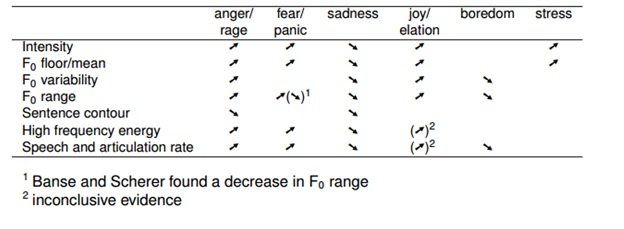
\includegraphics[scale=0.8]{emotion-table-example}
	\caption{Sound characterisstics for emotions [1]}
	\label{fig:emotion-table-example}
\end{figure}

For example, at the Figure 1 showed some features of emotions. And we can see that some emotions very similar(anger-joy,sadness-boredom). Although number of emotions is not so large. But with increasing number of emotions, also increases intersections between emotions on features. So it's important to define emotions which is needed for particular task
\end{document}
